%%%%%%%%%%%%%%%%%%%%%%%%%%%%%%%%%%%%%%%%%
% Medium Length Graduate Curriculum Vitae
% LaTeX Template
% Version 1.1 (9/12/12)
%
% This template has been downloaded from:
% http://www.LaTeXTemplates.com
%
% Original author:
% Rensselaer Polytechnic Institute (http://www.rpi.edu/dept/arc/training/latex/resumes/)
%
% Important note:
% This template requires the res.cls file to be in the same directory as the
% .tex file. The res.cls file provides the resume style used for structuring the
% document.
%
%%%%%%%%%%%%%%%%%%%%%%%%%%%%%%%%%%%%%%%%%

%----------------------------------------------------------------------------------------
%	PACKAGES AND OTHER DOCUMENT CONFIGURATIONS
%----------------------------------------------------------------------------------------

\documentclass[margin, 10pt]{res} % Use the res.cls style, the font size can be changed to 11pt or 12pt here

%!TEX encoding =  UTF-8 Unicode
\usepackage[utf8]{inputenc}

\usepackage{helvet} % Default font is the helvetica postscript font
%\usepackage{newcent} % To change the default font to the new century schoolbook postscript font uncomment this line and comment the one above

\usepackage{amsmath}
\usepackage{amssymb}
\usepackage{amsthm}
\usepackage{graphics}
\usepackage{tikz}
\usepackage[all]{xy}
\usepackage{verbatim} %para fazer coment�rios
\usepackage{graphicx}
\usepackage{graphics}
\usepackage{url}
\usepackage{hyperref}
\usepackage[export]{adjustbox}

\setlength{\textwidth}{5.1in} % Text width of the document

\begin{document}

%----------------------------------------------------------------------------------------
%	NAME AND ADDRESS SECTION
%----------------------------------------------------------------------------------------

\moveleft.5\hoffset\centerline{{\Huge\bf RA\'UL PENAGUI\~AO PhD.}} % Your name at the top
\vspace{1.5mm}
\moveleft.5\hoffset\centerline{{\it Mathematics researcher: optimization, algebra, geometry and combinatorics}}

\moveleft.5\hoffset\centerline{{\it  Math Olympiad prize winner. Software developer in C++, python and Macaulay2}}

\moveleft.5\hoffset\centerline{{ \it Principal instructor in advanced courses in mathematics, organizer of research conferences and workshops}} % Your name at the top

\begin{figure}
\centering
\begin{minipage}{.5\textwidth}
  \centering
  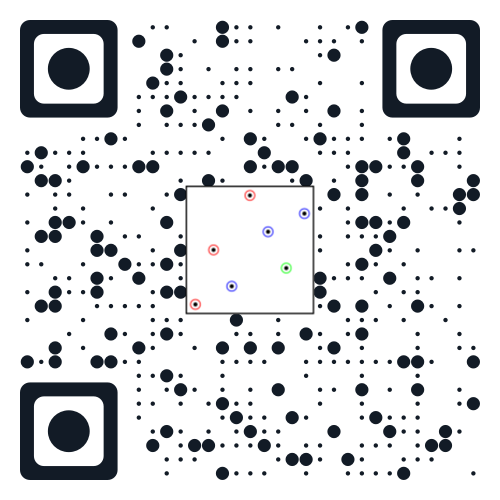
\includegraphics[width=.4\linewidth, left]{websiteQRcode.png}
\end{minipage}%
\begin{minipage}{.5\textwidth}
  \centering
  \includegraphics[width=.5\linewidth]{capaderevista2.jpg}
\end{minipage}
\end{figure}


%\begin{minipage}[b]{0.48\linewidth}
%%\centering
%\begin{flushleft} 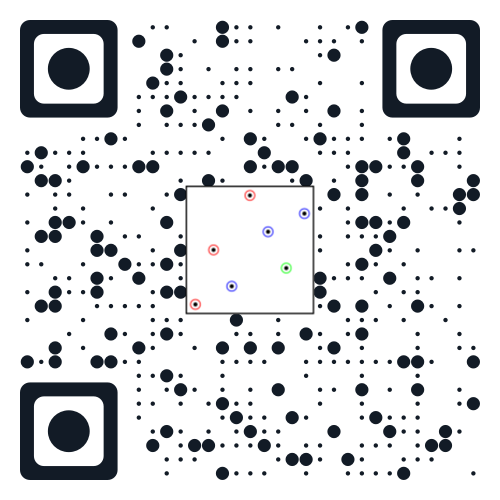
\includegraphics[scale=0.25]{websiteQRcode.png}
%\end{flushleft}
%\begin{flushright} \includegraphics[scale=0.25]{capaderevista2.jpg}
%\end{flushright}
%\end{minipage}
%\begin{table}[ht]
%\begin{tabular}{ll}
%\begin{flushleft} 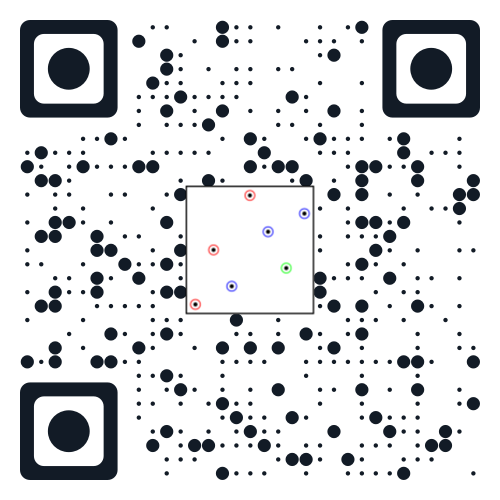
\includegraphics[scale=0.25]{websiteQRcode.png}
%\end{flushleft}
%&\hspace{5cm}\begin{flushright} \includegraphics[scale=0.25]{capaderevista2.jpg}
%\end{flushright}
%\end{tabular}
%\end{table}%
 
%\includegraphics{Capa_de_Revista.png}
 
\moveleft\hoffset\vbox{\hrule width\resumewidth height 1pt}\smallskip % Horizontal line after name; adjust line thickness by changing the '1pt'
 \vspace{-5mm}

\section{Contact}

\begin{table}[ht]
\begin{tabular}{l|l}
\href{https://orcid.org/0000-0002-0651-9036}{OrcID - \small{0000-0002-0651-9036}} & Personal website - \href{https://raulpenaguiao.github.io/}{raulpenaguiao.github.io} \\
Basel, Switzerland & Mail: rpenaguiao@haeusler.com \\
%Date of Birth: 30 - 12 - 1993 & Phone Contact : +41788030026 \\
Nationality: Portuguese & Github:  \href{https://github.com/raulpenaguiao}{raulpenaguiao}
\end{tabular}
\end{table}%



%----------------------------------------------------------------------------------------

\begin{resume}
\vspace{-5mm}
\moveleft\hoffset\vbox{\hrule width\resumewidth height 1pt}\smallskip % Horizontal line after name; adjust line thickness by changing the '1pt'
\vspace{-5mm}

%----------------------------------------------------------------------------------------

%----------------------------------------------------------------------------------------
\section{Employment}


{\sl Haeusler AG}, Basel, Switzerland. (September 2023 - Today)\\
Software engineer \href{https://haeusler.com/}{Haeusler AG}

{\sl Max Planck Institute}, Leipzig, Germany. (September 2022 - September 2023)\\
PostDoc researcher under the \href{https://www.mpg.de/en}{Max Planck society}\\
Graphical models in statistics, machine learning, algebraic geometry\\
Principal instructor in Algebraic Methods in Combinatorics \href{https://sites.google.com/view/amc-2023/home}{Link to webpage}

{\sl San Francisco State University}, San Francisco, US. (August 2021 - August 2022)\\
PostDoc researcher under the \href{https://www.snf.ch/en/f6JZyI4uQ1mNeq3J/funding/funding/discontinued-funding-schemes/early-postdoc-mobility}{Early.Postdoc Swiss National fund grant}\\
Combinatorial optimization, matroid theory, tropical geometry\\
Principal instructor in MATH 226 \href{http://bulletin.sfsu.edu/courses/math/}{Link to webpage}

%{\sl FU Berlin}, Berlin, Germany. (April 2021 - July 2021)\\
%PostDoc researcher under the \href{https://www.snf.ch/en/f6JZyI4uQ1mNeq3J/funding/funding/discontinued-funding-schemes/early-postdoc-mobility}{Early.Postdoc Mobility Swiss National fund grant}\\
%Polytopes, linear optimization, chromatic invariants


%{\sl University of Zurich}, Z\"urich, Switzerland. (September 2016 - August 2020)\\
%Teaching assistant and Doctoral student\\
%Algebraic combinatorics in Hopf algebra
{\small {\bf other employment: }}\\
{\small PostDoc researcher under a \href{https://www.snf.ch/en/f6JZyI4uQ1mNeq3J/funding/funding/discontinued-funding-schemes/early-postdoc-mobility}{Swiss National fund grant} at TU Berlin (2021)}\\
{\small Teaching assistant and doctoral student at University of Z\"urich (2016/202)}\\
{\small Teaching assistant at ETH Z\"urich (2015/2016)}\\
{\small Technical assistant at Novabase (2013/2014)}

%{\sl ETH Z\"urich}, Z\"urich, Switzerland.\\
%Teaching assistant\\
%Fall 2015 and Spring 2016
%
%
%{\sl NovaBase}, Lisbon, Portugal. - (Technical Assistant - October 2013 to January 2014)\\
%External Information: \url{http://www.novabase.pt/en}

\moveleft\hoffset\vbox{\hrule width\resumewidth height 1pt}\smallskip % Horizontal line after name; adjust line thickness by changing the '1pt'
\vspace{-5mm}

\section{Education}

{\sl University of Z\"urich}, Switzerland ( October 2016 - May 2020 )\\
Doctoral studies in mathematics - Degree (PhD) in Pure Mathematics \\
on \textit{Algebraic and geometric studies of combinatorial substructures and chromatic invariants}
PhD Advisor: Valentin F\'eray

{\sl ETH Z\"urich}, Switzerland (September 2014 - September 2016)\\
Masters of Science in Mathematics - Degree (MSc) in Pure Mathematics \\
Grade: 5.64/6 on \textit{The Chromatic Symmetric Function on Random Graphs} \\
Master Thesis advisors: Valentin F\'eray and Angelika Steger
 
%{\sl University of Lisbon}, Portugal. ( September 2011 - August 2014 )\\
%Degree (BSc) in Applied Mathematics and Computation. Grade: 19/20 \\
%Bachelor Thesis advisor: Miguel Abreu
 
%{\sl S. Maria Secondary School}, Sintra, Portugal.\\
%High School - Sciences and Technology\\
%September 2008 - June 2011
%----------------------------------------------------------------------------------------

%----------------------------------------------------------------------------------------
\moveleft\hoffset\vbox{\hrule width\resumewidth height 1pt}\smallskip % Horizontal line after name; adjust line thickness by changing the '1pt'


\section{Programming skills}

\begin{itemize}
\item General-purpose: C++, julia and Python
\item Technical computing systems: Mathematica, MatLab, SAGEmath, Macaulay-2
\item Markup languages: HTML and LaTeX
\end{itemize}
\vspace{-0.2cm}

\moveleft\hoffset\vbox{\hrule width\resumewidth height 1pt}\smallskip % Horizontal line after name; adjust line thickness by changing the '1pt'


\section{Institutional responsibilities}

Organizer of research seminar in the Fall semester 2021-2022, \textit{AGC}, at San Francisco State University - \href{https://sites.google.com/view/sfsuagc/fall-2021}{Web}.
\vspace{-0.2cm}

Organizer of AMS Spring Western Virtual Sectional Meeting at San Francisco State University, Sprint 2021 - \href{http://www.ams.org/meetings/sectional/2282_progfull.html}{Web}.
\vspace{-0.2cm}

Co-organizer of research Workshop in \textit{Permutation Patterns 2019}, at Z\"urich University - \href{https://sites.google.com/view/permutation-patterns-2019/pre-conference-workshop}{Web}.
\vspace{-0.2cm}

Representative of the teaching assistants in the committee of Mathematics department from 2017 January to 2017 June, University of Z\"urich.


\medskip

\moveleft\hoffset\vbox{\hrule width\resumewidth height 1pt}\smallskip % Horizontal line after name; adjust line thickness by changing the '1pt'

%
%
%\section{Research interests}  
%
%
%Patterns in permutations and related objects.
%
%Universal properties of symmetric functions in type A and B.
%
%Chromatic invariants on graphs, matroids, permutations and polytopes.
%
%%Graph theory, stable matchings and chromatic invariants;
%
%%Algebraic applications in combinatorics;
%
%%General topology and algebraic invariants;
%
%%Computer science, and applications of graph theory;
%
%
%\moveleft\hoffset\vbox{\hrule width\resumewidth height 1pt}\smallskip % Horizontal line after name; adjust line thickness by changing the '1pt'
%
%%\section{Favourite literature}  
%%
%%Aguiar, Marcelo, and Swapneel Arvind Mahajan. Monoidal functors, species and Hopf algebras. Vol. 29. Providence, RI: American Mathematical Society, 2010.
%%
%%Martin Aigner: Combinatorial Theory, 1979, \textit{Springer};
%%
%%Noga Alon, and Joel H. Spencer: The probabilistic Method 3rd edition, 2008, \textit{Wiley-Interscience};
%%
%%%Thomas W. Hungerford: Algebra, Graduate Texts in Mathematics v.73. Springer;
%%
%%%Bondy, John Adrian, and Uppaluri S. R. Murty, Graph theory with applications. 1976, \textit{London: Macmillan};
%%
%%%Frank W. Warner: Foundations of Differentiable Manifolds and Lie Groups, 1971, \textit{Springer};
%%
%%James R. Munkres: Topology, 2nd Edition, 2000, \textit{Pearson};
%%
%%\moveleft\hoffset\vbox{\hrule width\resumewidth height 1pt}\smallskip % Horizontal line after name; adjust line thickness by changing the '1pt'


\section{Selected scientific publications}


\begin{itemize}
%\item {\sl The kernel of chromatic quasisymmetric functions on graphs and nestohedra}, \textit{30th International Conference on Formal Power Series and Algebraic Combinatorics}.

\item {\sl The kernel of chromatic invariants on graphs and hypergraphical polytopes},  \href{https://www.sciencedirect.com/science/article/abs/pii/S0097316520300509?via%3Dihub}{Journal of Combinatorial Theory, Series A, 175, 105258}.

%
%\item {\sl Substructure algebras and marked permutations}, submitted for publication.

%\item {\sl Pattern Hopf algebras in presheaves}, in preparation.

%\item {\sl The feasible region for consecutive patterns of permutations is a cycle polytope}, \textit{32nd International Conference on Formal Power Series and Algebraic Combinatorics}.

\item {\sl  The tropical critical points of an affine matroid}, with Federico Ardila-Mantila and Christopher Eur, \small{\href{https://arxiv.org/abs/2212.08173}{To be published on SLC}.}

\item {\sl Pattern Hopf algebras}, \small{\href{https://link.springer.com/article/10.1007/s00026-022-00578-3}{Annals of Combinatorics volume 26, pages 405–451 (2022)}.}

\item {\sl The feasible regions for consecutive patterns of pattern avoiding permutations}, with Jacopo Borga, \href{https://doi.org/10.1016/j.disc.2022.113219}{Volume 346, Issue 2, February 2023, 113219}.

%\item {\sl Antipode formulas from the sign-reversion involution method}, with Yannic Vargas, in preparation.

%\item Coxeter variants of WQSym in Hopf monoids, and resulting chromatic problems. \textit{In preparation}.

\end{itemize}

\moveleft\hoffset\vbox{\hrule width\resumewidth height 1pt}\smallskip % Horizontal line after name; adjust line thickness by changing the '1pt'


%\section{Teaching experience}
%
%\textbf{Principal instructor} in 
%
%MATH 226 (calculus) - \href{http://bulletin.sfsu.edu/courses/math/}{Web}
%
%\textbf{Teaching assistant} in:
%
%Polytopes in 2020 fall semester - Federico Ardila - \href{http://bulletin.sfsu.edu/courses/math/}{Web}.
%\vspace{-.5cm}
%
%Probability II in 2019 fall semester - Valentin Féray - \href{https://www.math.uzh.ch/index.php?id=1402&key1=0&key2=3662&key3=282&semId=39&L=1}{Web}.
%\vspace{-.5cm}
%
%Stochastics in 2019 spring semester - Christoph Luchsinger - \href{https://www.math.uzh.ch/index.php?id=ve_vo_det&key1=0&key2=3448&semId=38}{Web}.
%\vspace{-.5cm}
%
%Linear algebra I in 2018 fall semester - Alberto Cattaneo - \href{https://www.math.uzh.ch/index.php?id=ve_vo_det&key2=3314&keySemId=37}{Web}.
%\vspace{-.5cm}
%
%Hopf algebras in 2018 spring semester - Benedict Stufler - \href{https://www.math.uzh.ch/index.php?id=ve_vo_det&key1=0&key2=3270&key3=564&semId=36&L=1}{Web}.
%\vspace{-.5cm}
%
%Probability II in 2017 fall semester - Valentin Féray - \href{https://www.math.uzh.ch/index.php?id=ve_vo_det&id=ve_vo_det&key1=0&key2=3059&key3=282&semId=35&L=1}{Web}.
%\vspace{-.5cm}
%
%Linear algebra II in 2017 spring semester - Andrew Kresch - \href{https://www.math.uzh.ch/index.php?id=ve_vo_det&id=ve_vo_det&key1=0&key2=2924&key3=468&semId=34&L=1}{Web}.
%\vspace{-.5cm}
%
%Mathematical foundations, 2016 fall semester - Mathilde Bouvel - \href{https://www.math.uzh.ch/index.php?id=ve_vo_det&id=ve_vo_det&key1=0&key2=2755&key3=234&semId=33&L=1}{Web}.
%\vspace{-.5cm}
%
%Analysis II in 2016 spring semester - \href{https://www2.math.ethz.ch/education/bachelor/lectures/fs2016/math/analysis2.html}{Web}.
%\vspace{-.5cm}
%
%Mathematica Methods in Physics I in 2015 fall semester - \href{https://www2.math.ethz.ch/education/bachelor/lectures/hs2015/math/mmp1.html}{Web}.
%
%
%\moveleft\hoffset\vbox{\hrule width\resumewidth height 1pt}\smallskip % Horizontal line after name; adjust line thickness by changing the '1pt'

%
%\section{Membership in panels and committees}
%
%Representation of the assistants in the Mathematics department for 2017 January to  2017 June.
%
%\medskip
%
%
%\moveleft\hoffset\vbox{\hrule width\resumewidth height 1pt}\smallskip % Horizontal line after name; adjust line thickness by changing the '1pt'

%\pagebreak

\section{Organization of conferences}

Organizer of the "NMath workshop for computer science and algorithms in 2021"
\vspace{-0.2cm}

Organizer of the "Student workshop for permutation patterns in 2019" - \href{https://sites.google.com/view/permutation-patterns-2019/pre-conference-workshop}{Web}.
\vspace{-0.2cm}

%\textit{This is a satellite workshop to the conference} \href{https://sites.google.com/view/permutation-patterns-2019}{Permutation Patterns 2019 - Zurich}.

Organizer of "Mathematics, Statistics and Computation Journeys" (JMEC 1), main organizer of the Math exposition in 2014 - \url{http://nmath.tecnico.ulisboa.pt/jm/}



\moveleft\hoffset\vbox{\hrule width\resumewidth height 1pt}\smallskip % Horizontal line after name; adjust line thickness by changing the '1pt'

%
%\section{Undergraduate scientific experience}
%
%
%\begin{itemize}
%\item {\sl Chromatic invariants on random graphs} (2016)\\
%Advisor: Valentin F\'eray, Z\"urich University.
%
%\item {\sl Chromatic invariants on graphs} (2015-2016)\\
%Advisor: Valentin F\'eray, Z\"urich University.
%
%%Mathematical research in the \textit{Mathematical youth talents} Program from Calouste Gulbenkian Foundation.
%
%\item {\sl Finite Quandles} (2013-2014)\\
%Advisor: Pedro Lopes, University of Lisbon.
%\item {\sl Dinitz conjecture, stable matching and graph painting} (2011-2012)\\
%Advisor: Jos\'e Fachada, University of Lisbon.
%\end{itemize}
%
%\moveleft\hoffset\vbox{\hrule width\resumewidth height 1pt}\smallskip % Horizontal line after name; adjust line thickness by changing the '1pt'


%\section{Seminars} 
%
%\begin{itemize}
%
%\item \textbf{From presheaves to Hopf algebras}, 82th Seminaire Lotharigien Combinatoire, Curia, (March, 2019).
%
%\item \textbf{Chromatic invariants in graphs and nestohedra}, Formal Power Series and Algebraic Combinatorics, Dartmouth USA, (July, 2018).
%
%\item \textbf{The kernel problem in graphs and nestohedra}, 80th Seminaire Lotharigien Combinatoire, Lyon, (March, 2018).
%
%\item \textbf{Chromatic functions on random graphs}, Discrete mathematics seminar, University of Zurich, (September, 2016).
%
%\item \textbf{Flips in triangulations}, Class seminar in "Geometry: Combinatorics and Algorithms", ETH Z\"urich, (May, 2015).
%
%\item \textbf{Non-repetitive Sequences in paths and graphs}, Mittagseminar, ETH Z\"urich, (May, 2015).
%
%
%\item \textbf{Quandle Structures On Knots}, Diagonal School, Universidade Nova de Lisboa, (February, 2014).
%
%\item \textbf{Stable Mariages on Bipartite graphs}, Diagonal School, Universidade Nova de Lisboa, (February, 2012).
%
%%Reference - \url{http://www.math.ist.utl.pt/~ggranja/Talentos/}
%
%%\item \textbf{Non-repetitive Sequences in paths and graphs}, Diagonal Seminar, Instituto Superior T\'ecnico, (June, 2015).
%
%%\item \textbf{Stable Mariages on Bipartite graphs}, Diagonal Seminar, Instituto Superior T\'ecnico, (March, 2012).
%
%%Reference - \url{https://math.ist.utl.pt/diagonal/index.php.pt};
%
%%\item \textbf{Topics on projective geometry}, Delfos Project, Coimbra University, (April, 2012).
%
%%\item \textbf{Applications of the Principle of inclusion-exclusion to IMO problems}, Delfos Project, Coimbra University, (November, 2011).
%
%%Reference - \url{http://www.uc.pt/fctuc/dmat/divulgacao/projetodelfos};
%
%%\item 20 years, 20 top mark - ISCTE Busines School, The influence of Mathematics (February 2013);
%
%%Reference - \url{http://www.tvi.iol.pt/programa/4790/artigos/6512}
%
%\end{itemize}
%
%%----------------------------------------------------------------------------------------
%
%%----------------------------------------------------------------------------------------
%\moveleft\hoffset\vbox{\hrule width\resumewidth height 1pt}\smallskip % Horizontal line after name; adjust line thickness by changing the '1pt'

\section{Awards and Fellowships}

{\sl Mathematical Olympiads}
\begin{itemize} \itemsep -2pt % Reduce space between items
\item Bronze Medal in the International Mathematical Olympiad. {\tiny 2011}
\item Silver medal in the Ibero-American Mathematical Olympiad for
University Students. {\tiny 2011}
\item Silver Medal in the Ibero-American Mathematical Olympiad. {\tiny 2011}
\item Three Gold Medals in the Portuguese Mathematical Olympiad. {\tiny 2008, 2010 and 2011}
%\item Silver Medal in the Portuguese Mathematical Olympiad. (2009)
%\item Honorable Mention in the International Mathematical Olympiad. (2009, 2010)
%\item Bronze medal in the Mayo Olympiads (2008).
%\item Gold medal in the Paulistas Olympiads (2008, 2009)
\end{itemize}

%{\sl Links}
%\begin{itemize}
%\item International Mathematical Olympiad link: http://www.imo-official.org/
%\item Portuguese Mathematical Olympiad link: http://www.spm.pt/olimpiadas/
%\end{itemize}

%%FALTA LINK DAS IBERO!!!
\vspace{-0.2cm}

{\sl Programming Team Olympiads}
\begin{itemize} 
\item Bronze Medal in South-West European Regional Contest. {\tiny 2011, 2012, 2013}
\item Gold Medal in the Portuguese Inter-Universitary Marathon. {\tiny 2011}
%\item Bronze Medal in the Portuguese Inter-Universitary Marathon. (2012, 2013)
\end{itemize} 
\vspace{-0.2cm}

%{\sl Links}
%\begin{itemize}
%\item South-West European Regional Contest. link: http://swerc.eu/
%\item Portuguese Inter-Universitary Marathon link: http://goo.gl/KZhlgk
%\end{itemize}

%{\sl Other Recognitions}
%\begin{itemize} 
%\item Civic Merith Medal - Silver - Sintra Town Council 2009/2010
%\item Scholar Merith Medal - Silver - S. Maria Secondary School 2008/2009
%\end{itemize} 


{\sl Fellowships}
\begin{itemize} 

\item Swiss national science foundation - PostDoc.Mobility grant {\tiny 2020 - 2022}

\item Calouste Gulbenkian foundation - \tiny{New talents fellowship. 2011-2012 and 2013-2014}
%\item Bronze Medal in the Portuguese Inter-Universitary Marathon. (2012, 2013)
%\item Calouste Gulbenkian foundation - New talents fellowship. (2013-2014)
\end{itemize} 

%----------------------------------------------------------------------------------------
%
%---------------------------------------------------------------------------------------- 
\moveleft\hoffset\vbox{\hrule width\resumewidth height 1pt}\smallskip % Horizontal line after name; adjust line thickness by changing the '1pt'


\section{Hobbies}

\begin{itemize}
\item Password manager. See \href{https://passworded.netlify.app/}{here}.
\item Clicker game. See \href{https://user.math.uzh.ch/penaguiao/Christmas_Game/}{here}.
\item Part of the scouting movement since five years old, still a volunteer
\item Hiking, camping and climbing (I have camped above 2800m altitude!)
\item Online programming competitions ($>330$ problems solved in Project Euler!)
\end{itemize}
\moveleft\hoffset\vbox{\hrule width\resumewidth height 1pt}\smallskip % Horizontal line after name; adjust line thickness by changing the '1pt'



%\section{Programs attended} 

%\begin{itemize}

%\item FPSAC London, 2017 and FPSAC Dartmouth, 2018;
%\item AEC Summer school, 2016 and AEC ;
%\item HackZ\"urich, Z\"urich, 2015;

%\item Olympic Week, by Brazilian Mathematical Society, Cutibar\'a, Brazil 2011;
%\item Olympic Week, by Brazilian Mathematical Society, Brazil 2010 and 2011;

%\item International Mathematical Summer School for students, Jacob's University, Bremen, Germany 2011;
%http://math.jacobs-university.de/summerschool/2011/

%\item Olympic Week, by Brazilian Mathematical Society, Rio Preto, Brazil 2010;
%\item London International Youth Science Forum, London 2012;
%\item Mathematical Summer School by Calouste Gulbenkian Foundation, Lisbon 2011 and 2012;
%\item Mathematical Summer School by Calouste Gulbenkian Foundation, Lisbon 2011;
%\item Delfos Project, form 2008 April, to 2011 September;

%\end{itemize}


%\moveleft\hoffset\vbox{\hrule width\resumewidth height 1pt}\smallskip % Horizontal line after name; adjust line thickness by changing the '1pt'

%\section{Language skills}

%Portuguese: Mother tongue.
%English: C.
%German: B2.
%French, Spanish: A2.


%\moveleft\hoffset\vbox{\hrule width\resumewidth height 1pt}\smallskip % Horizontal line after name; adjust line thickness by changing the '1pt'

%
%\section{Extra-curricular activities}
%
%{\sl BoyScout}, Carcavelos, Portugal. From 1999 to today.\\
%Instructor: December 2012 - Today\\
%Clan Guide: 2012 - 2013\\
%Clan treasurer: 2011 - 2012\\
%Stone-curlew patrol Secretary: 2005-2011\\
%External Information: \url{https://www.facebook.com/escoteiroscarcavelos} \\
%
%%{\sl Helper on the food bank - "Banco Alimentar contra a Fome"}, Carcavelos, Portugal. From 2005 to 2014.\\
%
%%----------------------------------------------------------------------------------------
%\moveleft\hoffset\vbox{\hrule width\resumewidth height 1pt}\smallskip % Horizontal line after name; adjust line thickness by changing the '1pt'
%
%\pagebreak
%
%
%\section*{Scientific works}
%
%\begin{itemize}
%
%\item Penaguiao, Raul. "The kernel of chromatic invariants on graphs and hypergraphical polytopes.", submitted for publication.
%
%This work is a proposed strategy to tackle the famous \textit{Stanley conjecture}, a 20 year old open problem in graph theory and algebraic combinatorics that has had remarkable attention and many partial solutions.
%I also related this conjecture as a \textbf{kernel problem}, a more general approach that allows me to look to related problems in other combinatorial objects, most remarkably generalized permutahedra.
%See on \href{https://arxiv.org/abs/1803.08824}{arxiv}.
%
%\item Penaguiao, Raul. "Substructure algebras: marked permutations, marked graphs and other combinatorial presheaves.", In preparation.
%
%The motivation for this work was the \textit{permutation patterns Hopf algebra}, a Hopf algebra constructed in the literature for permutations, shown to be free.
%I construct pattern Hopf algebras in general combinatorial objects, and establish the freeness for the class of \textbf{marked permutations} and for any class that has a \textbf{commutative product}, like posets or marked graphs.
%See my latests \href{https://user.math.uzh.ch/penaguiao/docs/Mathdocs/pper-draft.pdf}{preprint} in my homepage.
%
%\item Borga, Jacopo, and Penaguiao, Raul. "A polytope model for the consecutive occurrences of permutations.", In preparation.
%
%This work is an application of geometry and combinatorics of polytopes to the universe of random combinatorial objects.
%Specifically, for big permutations, we study the possible proportion of \textit{consecutive-patterns} of permutations.
%This forms, strikingly, a polytope.
%My experience with \textbf{polytopes} and \textbf{combinatorial techniques relating polytopes} was my contribution in this project. 
%See our latests \href{https://user.math.uzh.ch/penaguiao/docs/Mathdocs/patterns-and-polytopes-draft.pdf}{preprint} in my homepage.
%
%\end{itemize}
%
%
%\section*{Knowledge transfer events - talks} 
%
%\begin{itemize}
%
%\item \textbf{From presheaves to Hopf algebras}, 82th Seminaire Lotharigien Combinatoire, Curia, (March, 2019).
%
%\item \textbf{Chromatic invariants in graphs and nestohedra}, Formal Power Series and Algebraic Combinatorics, Dartmouth USA, (July, 2018).
%
%\end{itemize}

%
%\section*{Knowledge transfer events - organization of seminars} 
%
%\begin{itemize}
%
%
%\item "Student workshop for permutation patterns in 2019" organization - \href{https://sites.google.com/view/permutation-patterns-2019/pre-conference-workshop}{link}.
%My role was to contacting speakers, organize logistics and to apply for grants to fund the event together, with other organizers.
%
%\item "Mathematics, Statistics and Computation Journeys 2013" (JMEC) - \href{http://jmec.ist.utl.pt/}{link}.
%My role was to organize a museum type of exposition for mathematics geared to high school students.
%
%
%\end{itemize}


\end{resume}
\end{document}